
\section{Descriptions des besoins}


\begin{tabular}{|l|c|r|}
     \hline
    Liens & Besoin fonctionnels  & Priorité \\
    \hline
    3.1.1 & Plateau de Jeu & Élevée\\
    3.1.2 & API & Élevée\\ 
    3.1.3 & Unités & Élevée\\
    3.1.4 & Organisation de l'armée & Moyenne \\
    3.1.5 & Mouvement & Élevée \\
    3.1.6 & Combat & Élevée \\
    3.1.7 & Opérations Aériennes et Navales & Faible \\ 
    3.1.8 & Affichage & Élevée \\ 
    3.1.9 & Réseau  & Élevée \\
    \hline 
    
\end{tabular}

\begin{tabular}{l|c}
    \hline 
    Liens & Besoins non fonctionnels\\
    \hline
    3.2.1 & Affichage\\ 
    3.2.2 & Système\\
    \hline
\end{tabular}

Légende\\
\cmark : fait \\
\xmark : pas fait \\


\subsection{Besoins Fonctionnels}
\subsubsection{Plateau de Jeu}


\begin{itemize}
    \item \textbf{Priorité 3/3}
    \begin{itemize}
        \item Les hexagones numérotés, chacun représentant une distance définie, par défaut : 16 kilomètres \cmark
        \item Définir les joueurs et leurs spécificités. Par exemple les nationalités possibles, le joueur 
qui joue le premier et celui qui a l’initiative.\cmark
        \item Pouvoir poser des unités sur la carte et à retenir celles qui ne sont pas présentes dans
celles-ci \cmark
        \item Pouvoir poser plusieurs unités sur un hexagone.\cmark
        \item Être capable de faire des lancés de dés et d’appliquer des modificateurs. La majeure partie
du jeu se base sur les dés.\xmark
        \item Définir une séquence de tour :
        \begin{itemize}
            \item Pouvoir alterner entre les joueurs \cmark
            \item Respecter l’ordre strict d’un tour \cmark
        \end{itemize}
        \item Pouvoir déterminer quel joueur a l’initiative.
        \item Afficher un terminal qui permettra aux joueurs de donner des commandes d'attaque ou mouvement.\cmark
    \end{itemize}
    \item \textbf{Priorité 2/3}
    \begin{itemize}
        \item Différencier plusieurs types de terrain, les montages, les mers de sable et les crêtes
par exemple.\cmark
        \item Créer une base pour les cartes d’évènements. Celles-ci étant très différentes, l’implémentation sera limitée aux évènements génériques (non-spécifiques aux scénarios).\cmark
        \item Pouvoir charger la carte du jeu à partir d’un fichier \lstinline{txt} ou \lstinline{json} et pouvoir la sauvegarder
aux mêmes formats également.\cmark (mais pas la sauvegarde)
    \end{itemize}
    \item \textbf{Priorité 1/3}
    \begin{itemize}
        \item Ajouter les différents types d’indicateurs afin d’illustrer les villages, les villes et les
oasis par exemple. \cmark
    \end{itemize}
\end{itemize}

\subsubsection{API}
\begin{itemize}
    \item \textbf{Priorité 3/3}
    \begin{itemize}
        \item Pouvoir échanger des informations basiques entre serveur et client.\cmark
        \item Pouvoir convertir un état de la carte du jeu en format utilisable par le client pour pouvoir ensuite afficher le plateau.
        \item Envoyer un coup joue dans un format utile pour le serveur, pour pouvoir faire des éventuelles modifications sur le plateau.\cmark
        \item Vérification des coups :
        \begin{itemize}
            \item Envoyer le coup joue au serveur.\cmark
            \item Vérifier que le coup est valide.\cmark
            \item Retourner une réponse positive ou négative. Si le coup est bon alors envoyer le nouvel état de la carte du jeu au client.\cmark
        \end{itemize}
    \end{itemize}
\end{itemize}

\subsubsection{Unités}

\begin{itemize}
    \item \textbf{Priorité 3/3}
    \begin{itemize}
        \item Définir l'unité comme interface, qui aura une morale, peut être perturbée (disrupted) et qui peut prendre des actions basiques comme attaquer et bouger.\cmark
        \item Implémenter le système similaire à des points de vie (voir partie Depletion des règles).\cmark
        \item Séparer les unités en catégories différentes: motorisées, à pied, mécanisées, cavalerie etc.\cmark
        \item Mettre en place les situations ou l'unité devient perturbée :
        \begin{itemize}
            \item Trop de troupes sur un hexagone.
            \item Fin d'un mouvement de nuit.
            \item Après la phase de \"Supply Attrition\", il y a un échec sur le test d'usure (attrition).
        \end{itemize}
        \item Créer un système de zones de contrôle (ZDC):
        \begin{itemize}
            \item Pouvoir calculer si une unité peut exercer une ZDC.
            \item Choisir quel hexagone est dans cette ZDC.
            \item Appliquer des effets potentiels sur des unités présentes dans la ZDC.
            \item Permettre à certaines unités doit ignorer les ZDC dans certaines phases d'un tour
        \end{itemize}
    \end{itemize}
    \item \textbf{Priorité 2/3}
    \begin{itemize}
        \item Permettre aux unités éligibles de s'entraîner et de faire des upgrade.\xmark
    \end{itemize}
\end{itemize}

\subsubsection{Organisation de l'armée}


\subsubsection{Mouvement}
\begin{itemize}
    \item \textbf{Priorité 3/3}
    \begin{itemize}
        \item Le joueur du Commonwealth peut accélérer le mouvement de ses unités en utilisant le rail et transport maritime.\xmark
        \item Déplacement case par case, et enlever les points de mouvement correspondants de l'unité. Ceci pour limiter la capacité de mouvement.\cmark
    \end{itemize}
    \item \textbf{Priorité 2/3}
    \begin{itemize}
        \item Déplacement d'un point A à un point B, en parcourant le plus cours chemin
            On utilisera l'algorithme \emph{Dijkstra} pour satisfaire la condition.\cmark
        \item Appliquer un bonus de mouvement dépendant du terrain d'un hexagone. C'est plus facile de se déplacer sur une plaine plutôt qu'à travers des montagnes.
        \item Permettre aux unités qui doivent se replier de bouger de 1-3 hexagones. Ce mouvement ne coûte pas de points de mouvement.\cmark
        \item Ajouter la mécanique du overrun (fuite). Les unités capables de le faire peuvent pendant leur phase de mouvement attaquer des unités. Les défenseurs alors peuvent utiliser leurs phases de réaction pour bouger un certain nombre d'hexagones. La distance est définie par l'unité concernée.\xmark
    \end{itemize}   
    \item \textbf{Priorité 1/3}
    \begin{itemize}
        \item Mouvement la nuit.
    \end{itemize}
\end{itemize}

\subsubsection{Combat}
\begin{itemize}
    \item \textbf{Priorité 3/3}
    \begin{itemize}
        \item Pouvoir définir les unités participant au combat de ce round.
        \item Pouvoir déterminer la puissance de combat de l'armée composée de ces unités.
        \item Définir les règles du combat, par exemple le fait que seules les unités/armées adjacentes peuvent entrer en combat,par la volonté de l'attaquant.
        \item Pouvoir simuler le combat et donner les résultats.
        \begin{itemize}
            \item Déterminer les dégâts causés par une unité en divisant les points d'attaque par les points de défense de l'ennemie pour obtenir un ratio.
            \item Séparer les défenseurs en groupe de morale. Les unités avec la même morale se retrouvent dans le même groupe. Les résultats seront fais dans l'ordre descendant de morale. Par exemple si on a deux groupes de morale (de 1 et 2), alors les résultats du combat seront d'abord appliqués dans le groupe avec une morale de 2, puis a celui de morale 1.
            \item Appliquer des éventuelles règles spéciales.
            \item Si un hexagone contient que des unités de support, alors lancer un dé si l'attaquant le souhaite, pour tenter de capturer les unités. Un résultat de 1-3 est un succès et un résultat de 4-6 veut dire que les unités de support sont détruites.
            \item Amasser les dégâts et puis causer des dégâts aux unités adverses. Les dégâts sont divis jusqu'à que le maximum d'unités ait reçu un point de dégât, puis infliger les deuxièmes points de dégâts sur les unités, s'il reste des points de dégâts à distribuer.
            \item Enlever du plateau les unités détruites, et les ajouter dans la liste d'unités détruites du joueur concernée.
            \item Lancer un dé pour faire le test de morale des unités qui reste. Si le test échoue, alors l'unité est \"disrupted\".
        \end{itemize}
        \item Pouvoir simuler la retraite d'une armée si les spécifications le permettent, par exemple le terrain et la condition de l'armée est convenable, et si l'utilisateur le souhaite.
    \end{itemize}
    \item \textbf{Priorité 1/3}
    \begin{itemize}
        \item Si un Hex contient plusieurs terrains, le défendant doit pouvoir en choisir un pour sa défense.
    \end{itemize}
\end{itemize}

\subsubsection{Opérations Aériennes et Navales}
\begin{itemize}
    \item \textbf{Priorité 1/3}
    \begin{itemize}
        \item Pouvoir déterminer les différentes unités aériennes et navales ainsi que leurs spécificités.\xmark
        \item Pouvoir déterminer les différentes cibles, comme par exemple des bases militaires ou les rivages(pour les opérations navales surtout), qu'ils peuvent cibler et attaquer.\xmark
        \item En ce qui concerne les opérations navales, ils peuvent effectuer des expéditions transportant des munitions ainsi que des unités/machines de guerre.\xmark
    \end{itemize}
\end{itemize}

\subsubsection{Affichage}
\begin{itemize}
    \item \textbf{Priorité 3/3}
    \begin{itemize}
        \item Afficher le joueur dont c'est le tour.\cmark
        \item Déterminer et afficher les informations de fin de partie et du vainqueur.
        \item Afficher les différents marqueurs sur l'état de chaque composante du jeu, par exemple hors d'approvisionnement pour les unités.\cmark
        \item Afficher le résultat et les informations à la fin du combat.\cmark
    \end{itemize}
\end{itemize}

\subsubsection{Réseaux}
\begin{itemize}
    \item \textbf{Priorité 3/3}
    \begin{itemize}
        \item Le jeu sera autour d'une architecture client-serveur qui puisse se déployer à travers Internet (pas seulement sur un réseau local).\cmark
    \end{itemize}
\end{itemize}

\subsection{Besoins Non-Fonctionnels}

\subsubsection{Affichage}
\begin{itemize}
    \item Affiche un message d'erreur ou de refus quand une requête ou commande invalide est entrée.\cmark
    \item Mettre en place une interface graphique affichant le plateau du jeu, les unités.\cmark
    \item Afficher un message d'attente au joueur  qui ne joue pas .\cmark
\end{itemize}

\subsubsection{Système}
\begin{itemize}
    \item Le temps d'attente entre un coup proposé et sa validité évalué devront être de l'ordre de la seconde.\cmark
    \item Un chat sera créé pour communiquer avec l'adversaire.\cmark
\end{itemize}

\section{Scénario}

Les joueurs devront se connecter sur un serveur afin d'accéder à la partie. Le serveur hébergera la partie en traitant les mécanismes de la partie en arrière-plan. Les utilisateurs recevront une interface graphique en provenance du serveur et communiqueront avec cette interface pour jouer dans la partie.
Le serveur avertira l'utilisateur lors d'une mauvaise utilisation de l'interface et des requêtes parasites pour le serveur.


\begin{figure}[H]
\centering
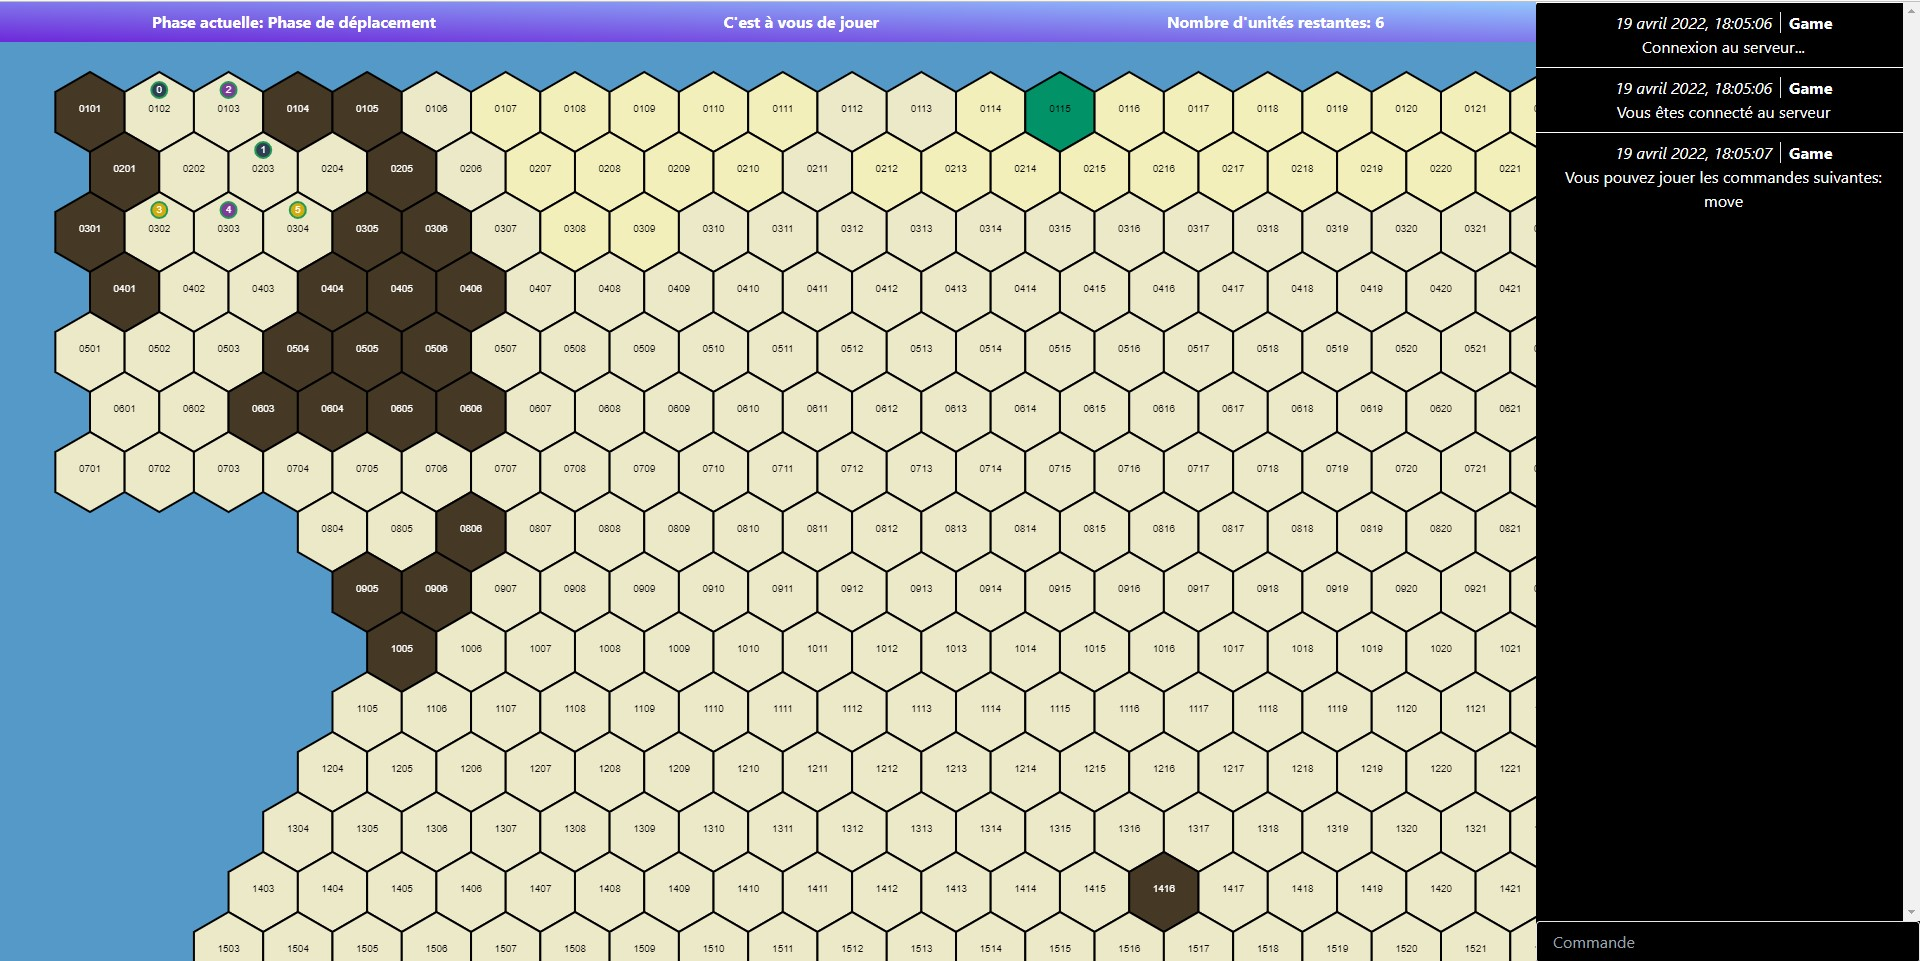
\includegraphics[scale=0.35]{data/plateau_du_jeu.jpg}
\caption{Plateau du jeu Desert Fox}.
\end{figure}

La carte s'affiche quand les deux joueurs sont connectés. Ici le joueur 1 peut commencer à jouer
. On peut voir en haut de la page, une barre qui affiche la phase actuelle sur 19, le tour  et le nombre d'unités restantes.


\begin{figure}[H]
\centering
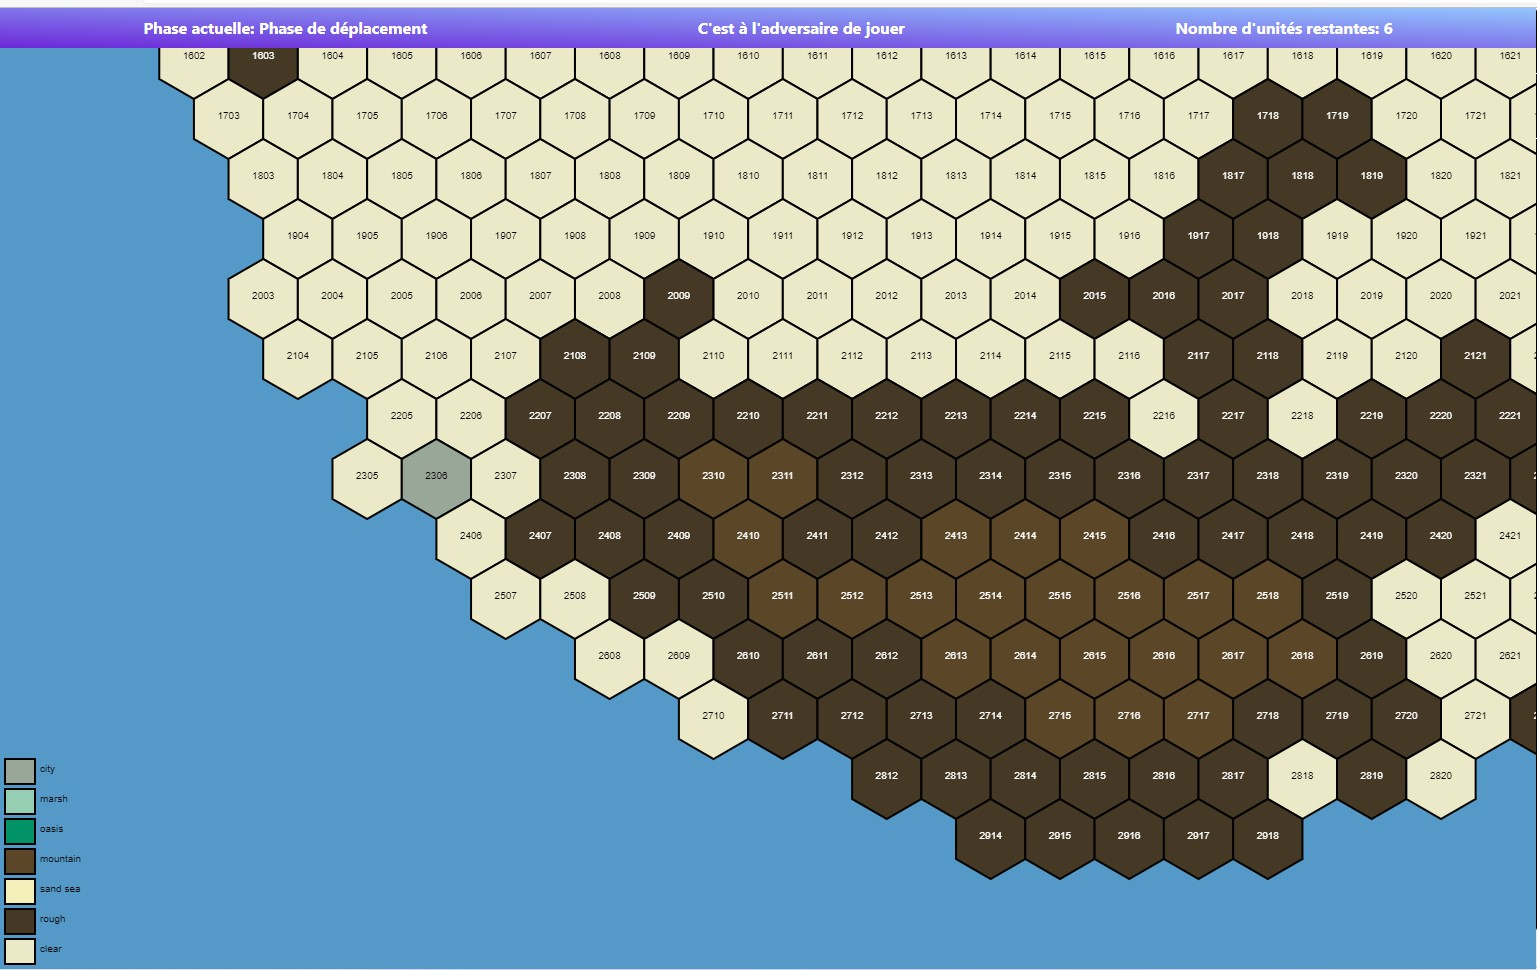
\includegraphics[scale=0.35]{data/justification2.jpg}
\caption{Bas de la carte et légende de la carte du jeu}.
\end{figure}
En bas de la carte, on peut observer une légende, en bas à gauche.\\
\begin{figure}[H]
\centering
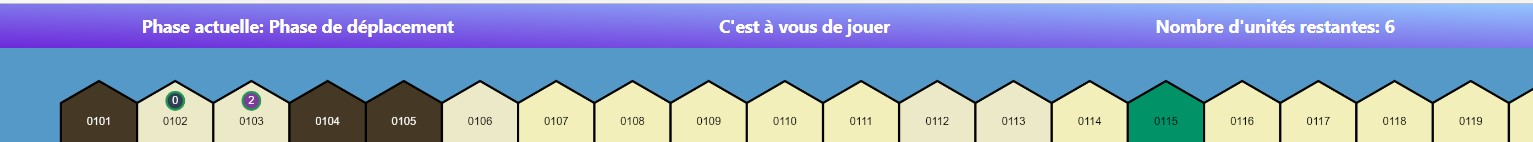
\includegraphics[scale=0.4]{data/player_1_acces.jpg}
\caption{Barre d'information du joueur 1}.
\end{figure}

Voici la page du joueur 1 qui peut jouer.\\

\begin{figure}[H]
\centering

\includegraphics[scale=0.35]{data/joueur_2.jpg}
\caption{Barre d'information du joueur 2}.
\end{figure}

Voici la page du joueur 2 qui doit attendre l'adversaire de jouer.

\begin{figure}[H]
\centering
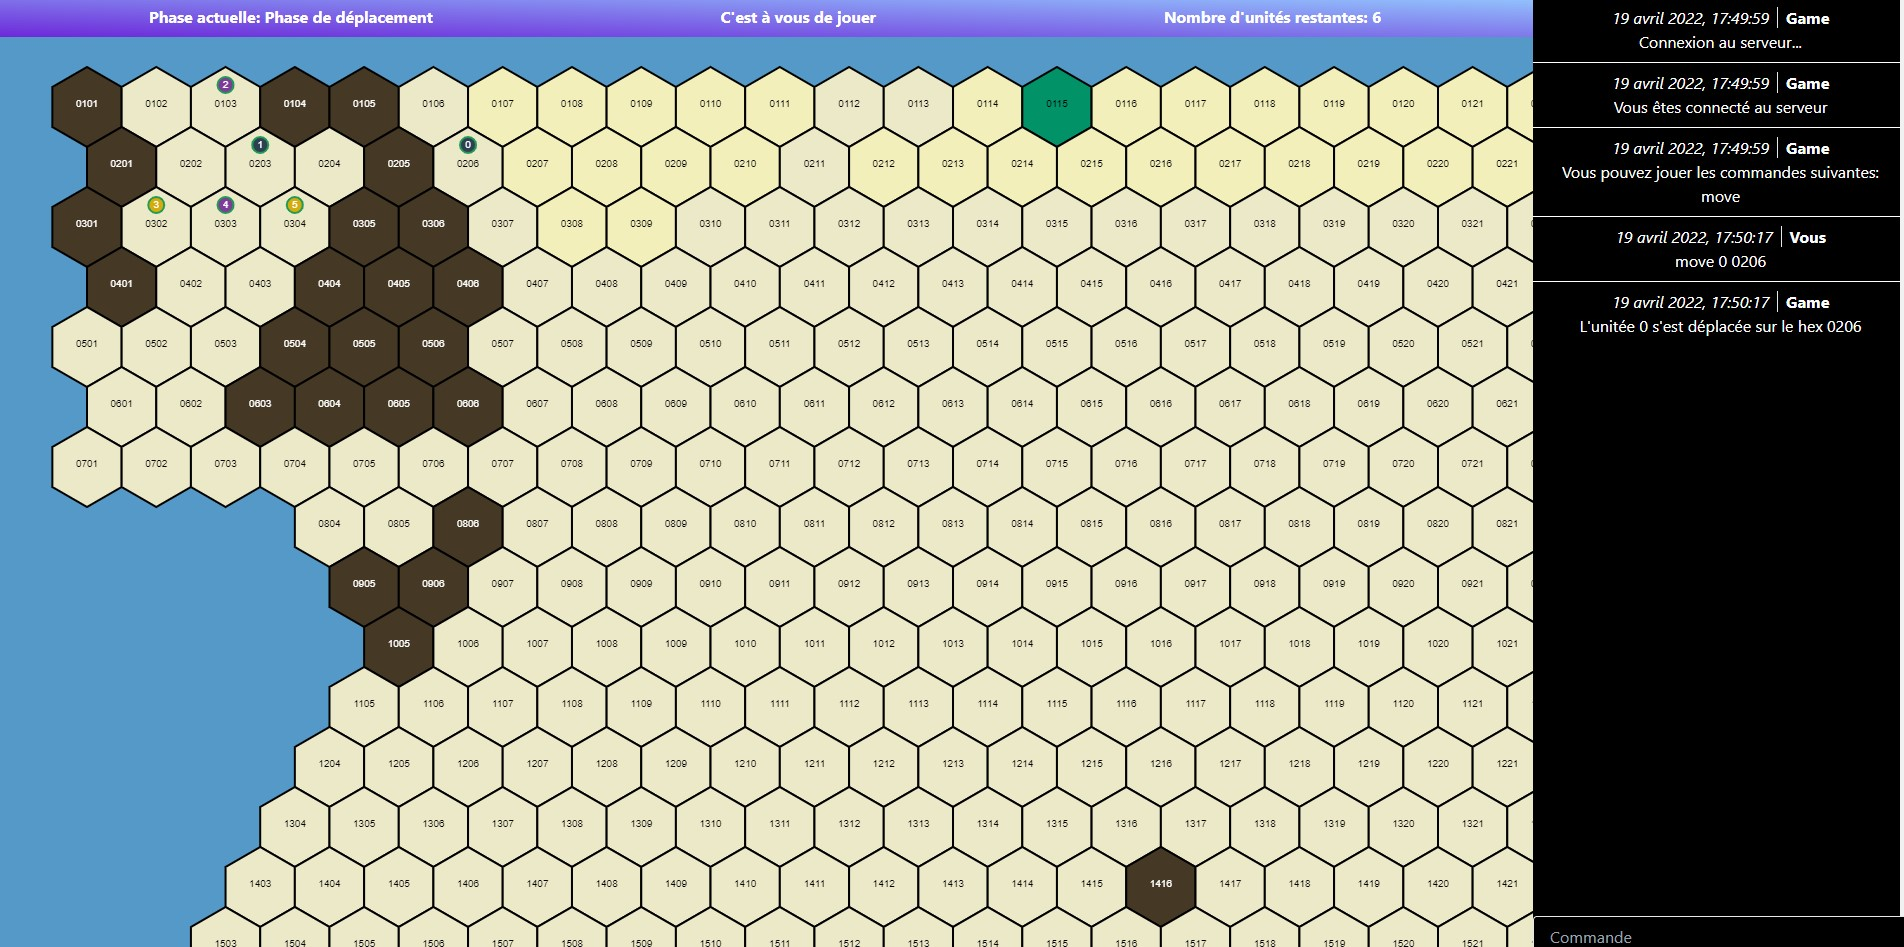
\includegraphics[scale=0.35]{data/move_unit_player_1.jpg}
\caption{Mouvement de l'unité \lstinline{0} vers l'hexagone \lstinline{0206}}.
\end{figure}

Le joueur qui peut jouer peut faire bouger son unité dans le terminal a droite de l'image.
On peut voir que l'unité 0 s'est déplacé de l'hexagone \lstinline{0102} à \lstinline{0206}. Le déplacement est valide car on ne dépasse pas le mouvement alloué de l'unité (MA).\\

\begin{figure}[H]
\centering
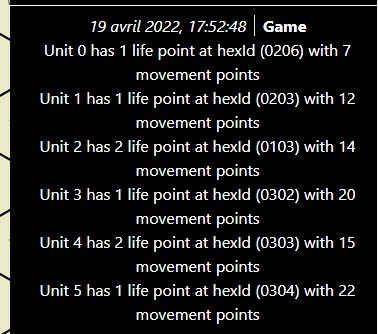
\includegraphics[scale=0.6]{data/info_units.jpg}
\caption{Terminal qui donne les informations des unités du joueur 1 }.
\end{figure}

Le joueur peut afficher des informations concernant ses unités dans le terminal.
En tapant \og units \fg{}, le joueur à toutes ses unités présent avec le mouvement point et  les points de vies.

\begin{figure}[H]
\centering
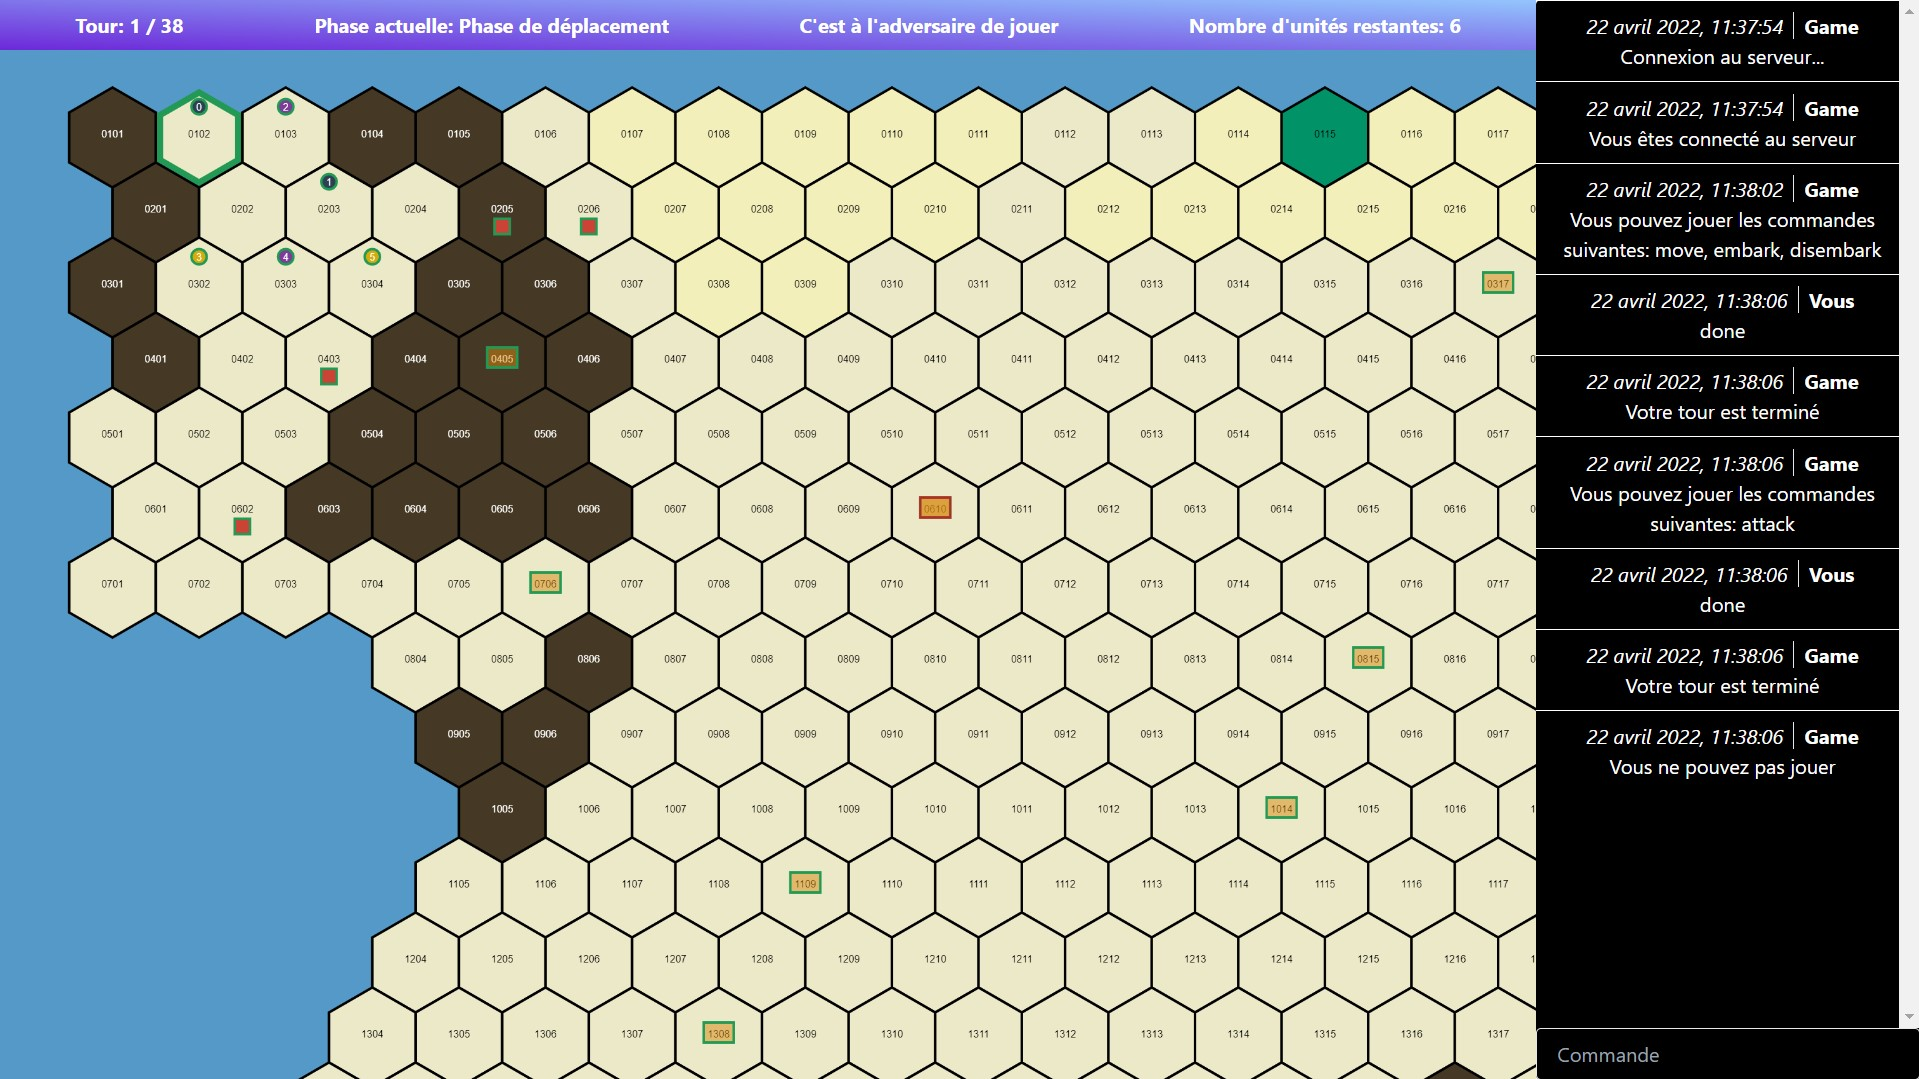
\includegraphics[scale=0.35]{data/fin_tour.jpg}
\caption{Fin du tour pour le joueur 1}.
\end{figure}

Quand le joueur a terminé son tour, il doit écrire dans le terminal \og done \fg{}
le joueur ne pourra que communiquer par chat à l'adversaire et l'adversaire peuvent continuer à jouer.\\

\begin{figure}[H]
\centering
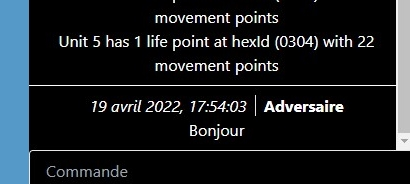
\includegraphics[scale=0.6]{data/chat.jpg}
\caption{Communication entre deux joueurs}.
\end{figure}
Les deux joueurs peuvent communiquer ensemble  à l'aide du terminal, le joueur doit écrire au dans le terminal \og message \fg{} puis écrit son message.


\begin{figure}[H]
\centering
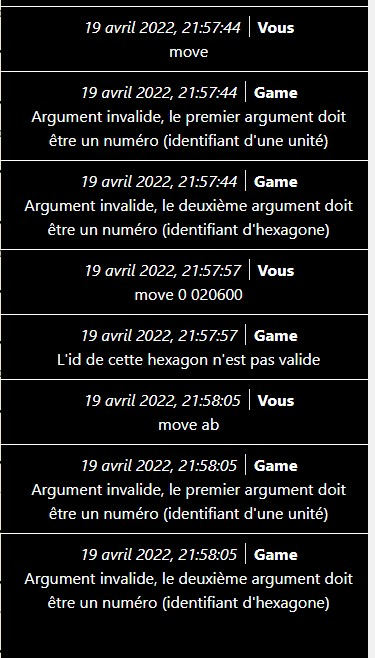
\includegraphics[scale=0.6]{data/erreur.jpg}
\caption{Exemple de mauvaises commandes}.
\end{figure}
Un message d'erreur s'affiche dans le terminal si le joueur écrit  des mauvaises commandes.
Par exemple, le joueur oublie les arguments, ou donne un mauvais hexagone.

